\section{Discussion}
Since the method outlined in this paper did not produce the predicted results and our hypothesis hence remains unproven, a deeper discussion of the apparant failure is of high interest. A correlation between $V_{in} = 5V$ and $V_{out} \approx 5V$ was quickly made, leading to the assumption that some sort of short between $V_{in}$ and $V_{out}$ had occured, the investigation ensued. The thick layer of (non-conducting!) hot-glue, earlier applied as a mechanical safety procedure after repeated pin header related failures, was carefully removed using a flat head screwdriver and rigorus amounts of determination. On closer inspection of the PCB, a short between $V_{in}$ and $V_{out}$ was observed, see Fig.\ref{fig:short}

\begin{figure}
    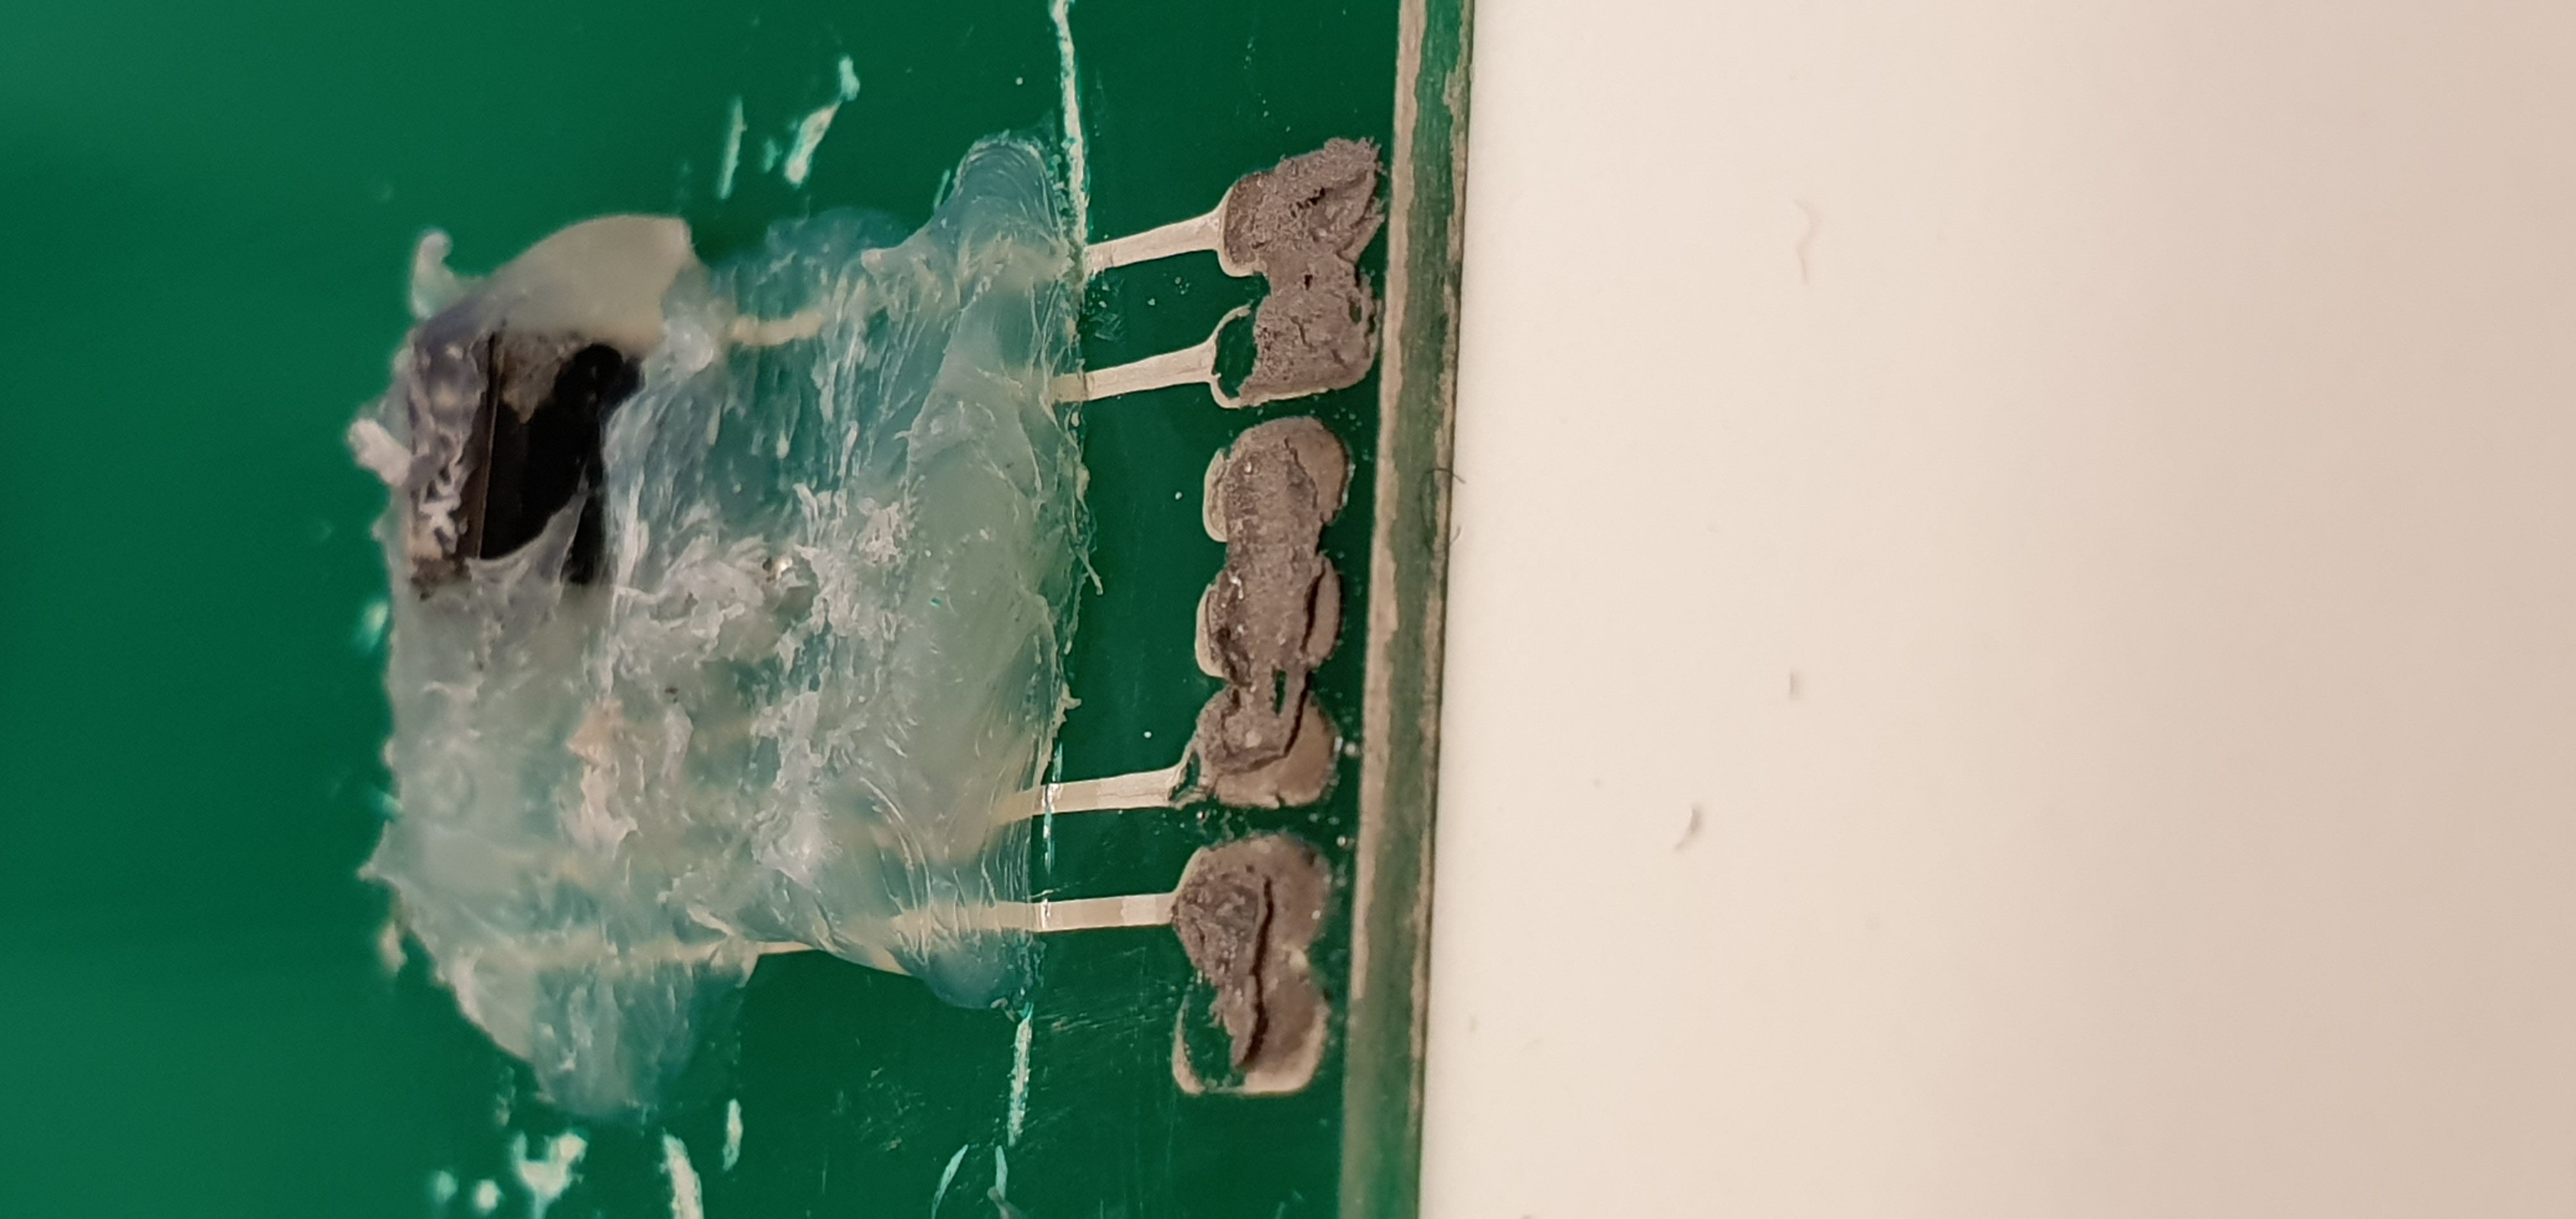
\includegraphics[width=\linewidth]{ela302-kortslutning.jpg}
    \caption{Picture of a short on the pin header.}
    \label{fig:short}
\end{figure}
